\section{Schlussteil}

\subsection{Probleme}

Die Verwendung von GWT für die Umsetzung des Projekts verlief überwiegend problemlos. Dennoch sind uns einige Aspekte aufgefallen, die etwas zu wünschen übrig ließen. Das betrifft zum einen den HTML-Code der Widgets und zum anderen die Abstraktionsmöglichkeiten von GSS.

\subsubsection{HTML-Code der Widgets}

In GWT werden Panels verwendet um das Layout der Anwendung zu definieren. Wir haben in unserem Projekt
hierzu überwiegend Horizontal-, Vertical- und FlowPanels verwendet. Neben diesen wurden für Tabellenstrukturen wie die Playlist
Flex- bzw. CellTables eingesetzt.

Bei der Analyse von Problemen bzgl. des Layouts und dem Styling von einzelnen Oberflächenelementen haben wir
festgestellt, dass die meisten Panels als verschachtelte <table>-Elemente im DOM eingefügt werden.
Dabei werden selbst einfache Panels in mehrfach verschachtelte HTML-Tabellen übersetzt (s. Abbildung \ref{fig:Probleme-HTML-tables}). Dies erschwert die Analyse von Layout und Styleproblemen, da im HTML-Code nicht direkt ersichtlich ist, ob die GWT-Elemente in <table>-Elemente übersetzt werden bzw. welches <table>-Element welchem GWT-Widget entspricht. 

\begin{figure}[htb]
\centering
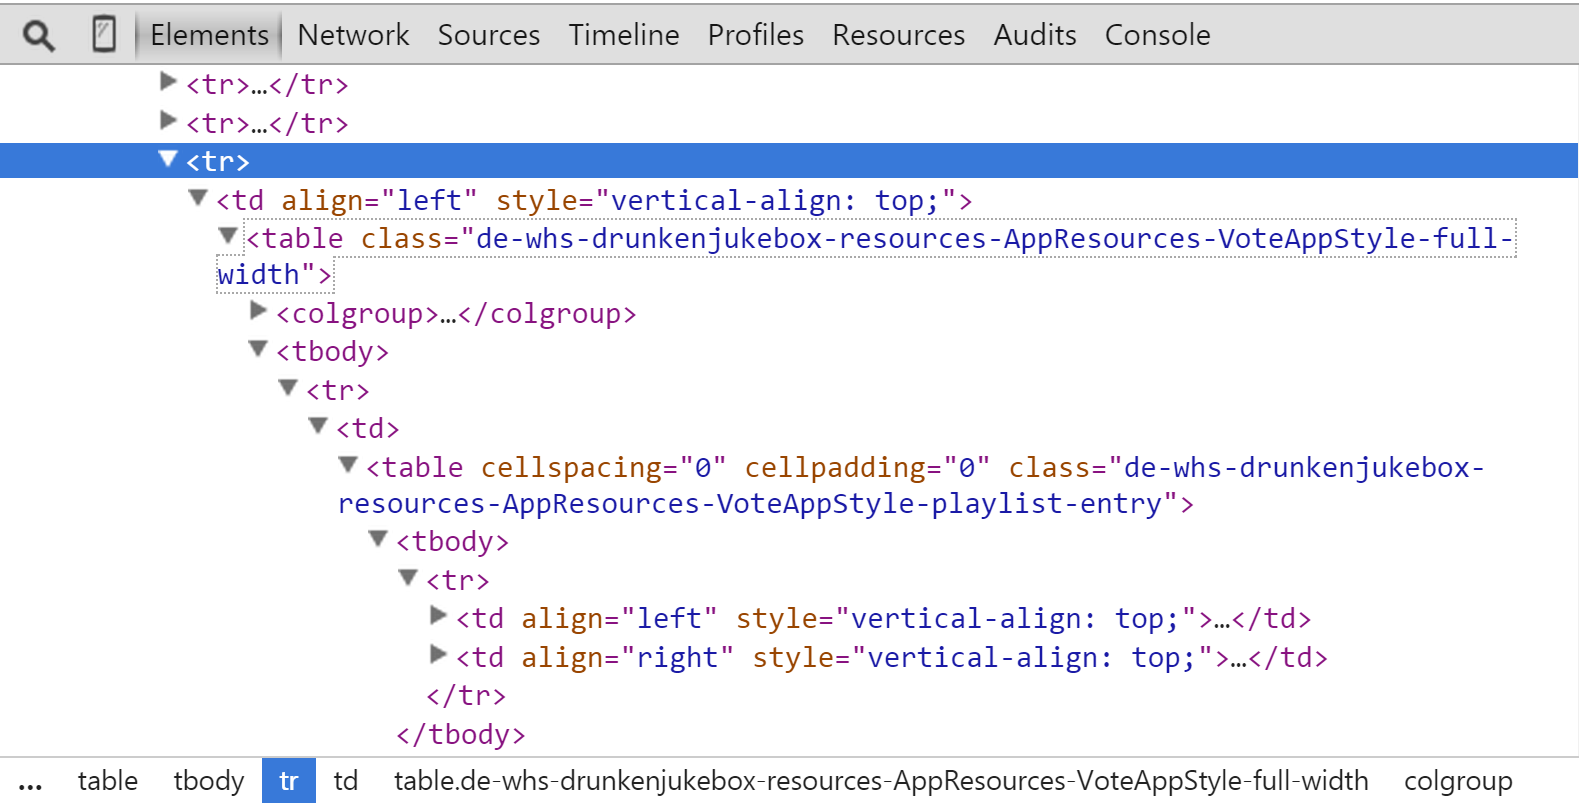
\includegraphics[width=1.0\linewidth]{Bilder/Probleme-HTML-tables}
\caption{Tabellenstruktur der VoteApp in den Chrome DevTools}
\label{fig:Probleme-HTML-tables}
\end{figure}

Aus den oben genannten Gründen haben wir zu Analysezwecken Styles auf verschiedene GWT-Widgets angewendet,
um ein Gefühl dafür zu bekommen, an welcher Stelle in der HTML-Tabellenstruktur diese eingefügt werden.
Wir hätten uns hier eine einfachere Übersetzung eines Layout-Widgets in z.B. genau ein <div>-Element gewünscht.
Damit wäre der Übersetzungsprozess von Widgets in HTML-Elemente besser nachvollziehbar 
und die Analyse von Fehlern beim Layout oder beim Styling wesentlich vereinfacht.
Es ist allerdings schwer zu beurteilen, ob andere Gründe für die Verwendung der Tabellenstruktur in GWT sprechen.
 
\subsubsection{Zu geringe Abstraktionsmöglichkeiten in GSS}

Bei der Verwendung von GSS ist uns aufgefallen, dass die gegebenen Abstraktionsmöglichkeiten
für bestimmte Anwendungsfälle nicht ausreichen. In unserem Projekt betrifft das die Definition
von Button-Styles.
Da unsere Buttons einheitlich aussehen sollten und sich lediglich in der Farbe unterscheiden, 
haben wir Mixins in GSS genutzt um die CSS-Eigenschaften zu abstrahieren. Als Parameter kann
die Hintergrund- sowie die Randfarbe angepasst werden.

\begin{lstlisting}[language=CSS]
@defmixin coolButton(BACKGROUND, BORDER) {
  color: BUTTON_TEXT_COLOR; 
  background-color: BACKGROUND; 
  border-color: BORDER; 
  /* ... */
}
\end{lstlisting}

Für die Definition eines Styles reicht diese Abstraktion. Wir wollten allerdings Buttons mit unterschiedlichen Farben definieren. Da sich das Aussehen eines Buttons ändert, wenn er aktiv ist oder sich
die Maus über diesem befindet, sind einzelne CSS-Anweisungen notwendig.

\begin{lstlisting}[language=CSS]
.up-vote { 
  @mixin coolButton(OK_BUTTON_COLOR, OK_BUTTON_BORDER);
  /* ... */
} 

.up-vote:hover, 
.up-vote:focus, 
.up-vote:active
{ 
  @mixin coolButton(OK_BUTTON_ACTIVE, OK_BUTTON_BORDER);
  /* ... */
} 
\end{lstlisting}

Um davon ausgehend einen Button mit einer anderen Farbe anzulegen, muss dieser Code kopiert und
die Farbparameter angepasst werden.
Das ist notwendig, da GSS keine Abstraktionsmöglichkeit zur Generierung mehrerer CSS-Deklarationen
bietet. Ein Mixin kann nur CSS-Eigenschaften in einer Anweisung erzeugen.

Dieses Problem wird von \textit{less} über "`Nested Rules"' und "`Parent Selectors"' gelöst\footnote{\url{http://lesscss.org/features/\#parent-selectors-feature}}. Ein ähnliches Konzept
hätten wir uns auch in GSS gewünscht.

\subsection{Ausblick}
Im Verlauf des Projekts haben sich weitere Ideen entwickelt, die wir leider aus zeitlichen Gründen nicht mehr umsetzen konnten. Anwendungsübergreifend hätten wir gerne Tests implementiert, um diesbezüglich Erfahrung im GWT-Umfeld zu sammeln. 

Für die Admin-Applikation wäre die Möglichkeit eines batchartigen Musikimports mehr als wünschenswert. Auf Seiten der VoteApp gibt es eine ganze Reihe von Verbesserungs- und Erweiterungsideen. Grundsätzlich sollte die VoteApp für die Nutzung auf einem Smartphone optimiert werden. Im diesem Zusammenhang könnten weitere visuelle Effekte beispielsweise für die Veränderung der Song-Rangliste hinzugenommen werden, um die Anwendung ansprechender zu gestalten. Darüber hinaus muss die Anwendung auf den wichtigsten mobilen Betriebssysteme lauffähig sein, was beispielsweise den Einsatz von PhoneGap erfordert. Die Bedienbarkeit muss dazu so angepasst werden, dass sie allen Design-Richtlinien entspricht. Beispielweise könnte in diesem Zusammenhang der Dialog, der zur Eingabe des DI-Wertes dient, durch dynamische Elemente ersetzt werden. 

Bezüglich des Drunken-Index besteht des Weiteren die Idee, statt des Sliders den DI auf anderem Wege zu ermitteln. Eine Art Spiel, anhand dessen sich ein Wert auf der Betrunkenheitsskala ermitteln lässt, wäre vorstellbar. Unabhängig davon sollte jedoch in jedem Fall der Partygast motiviert werden seinen DI regelmäßig einzureichen. Es wäre ein Punktesystem denkbar, bei dem es für die Eingabe des DIs Punkte gibt, die bei Abgabe eines Votes verbraucht werden. Neben den vorgestellten Ideen sind selbstredend noch viele weitere Innovationen vorstellbar.

\subsection{Fazit}
Im Verlauf des MWB-Projekts wurden zwei Anwendungen in GWT implementiert, die über einen Proxy mit dem Backend auf Basis von Deployd als Alternative zum WildFly kommunizieren. Sowohl die Anwendung für den Administrator als auch die App für die Partygäste erfüllen alle eingangs spezifizierten Anforderungen. Unter der Verwendung von MVP haben wir zahlreiche eigene Widgets entwickelt, die in beiden Anwendungen genutzt werden. Die Vorteile von MVP sind allerdings aufgrund der geringen Komplexität unseres Projekts nicht deutlich geworden. 

Die Verwendung von GWT und den dazu gehörigen Erweiterungen verlief für ein so großes Framework erstaunlicherweise problemlos.
So brachte beispielsweise ein Upgrade der GWT-Version von 2.6 auf 2.7 zur Mitte unseres Projekts keinerlei Probleme mit sich. Zudem stehen eine sehr große Auswahl der wichtigsten Oberflächenkomponenten bereits im Standard zur Verfügung, jedoch haben uns weitergehende Komponenten wie beispielsweise der Slider gefehlt. Bei dessen Implementierung waren wir positiv über den einfachen Einsatz von JSNI ohne erwähnenswerte Komplikationen überrascht. Ebenso gut hat uns das Grundprinzip von GSS gefallen, wobei wir wie beschrieben teilweise weitergehende Abstraktionsmöglichkeiten vermissen.

Insgesamt hat das Projekt gezeigt, dass GWT ein gutes Tool ist, welches zum Einsatz in produktiven Umgebungen geeignet ist. Wir sind abschließend mit unserem Projekt und den Möglichkeiten von GWT zufrieden.

